We have been writing the missing manual for peer-produced peer learning:
the ``Peeragogy Handbook''
(\href{http://peeragogy.org/}{peeragogy.org}). Throughout this work we
have asked and aimed to address questions like these:

\emph{What would a motivated group of self-learners need to know to
agree on a subject or skill to learn, find and qualify the best learning
resources about that topic, then select and use appropriate
communication media to learn it together? What would these people need
to know about learning to put together a successful learning programme?}

It is clear to us that the techniques of `peer production' that have
built and continue to improve Wikipedia and GNU/Linux have yet to fully
demonstrate their power in education. We believe that the Peeragogy
Handbook can help change that by building a distributed community of
peer learners/educators, and a strongly vetted collection of best
practices. Our project complements others' work on sites like
Wikiversity and P2PU, and builds upon understandings that have developed
informally in distributed communities of hobbyists and professionals, as
well as in (and beyond) the classrooms of generations of passionate
educators.

Here, we present Peeragogy in Action, a project guide in 4 parts. Each
part relates to one or more sections of our handbook, and suggests
activities to try while you explore peer learning. These activities are
designed for flexible use by distributed groups, collaborating via a
light-weight infrastructure. Participants may be educators, community
organisers, designers, hackers, students, seasoned peeragogues, or first
timers. The guide should be useful for groups who want to build a strong
collaboration, as well as to facilitators or theorists who want to hone
their approach. Together, we will use our various talents to build
effective methods and models for peer produced peer learning. Let's get
started!

\begin{center}
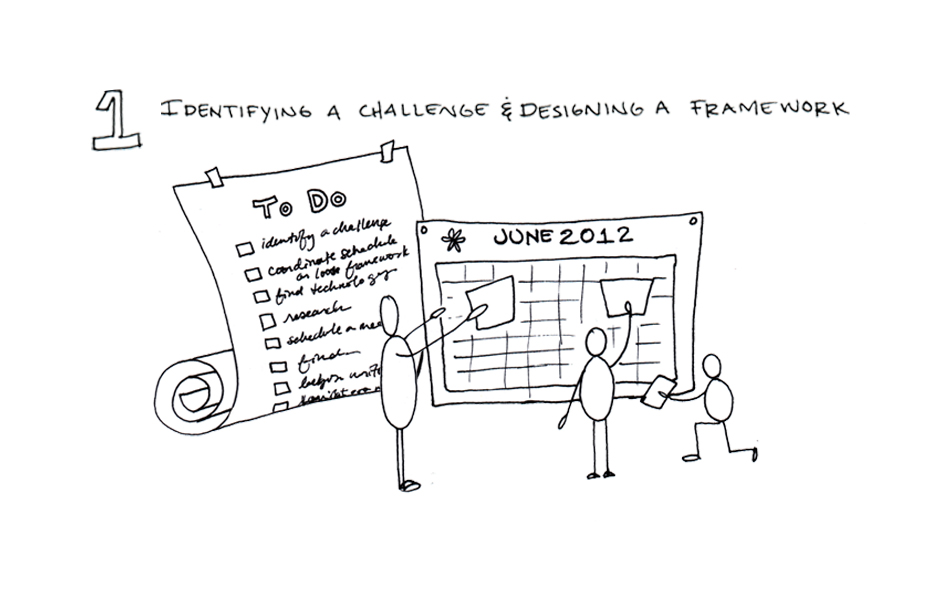
\includegraphics{./pictures/OpenBook-2-1.jpg}
\end{center}

\textbf{Setting the initial challenge and building a framework for
accountability among participants is an important starting point.}

\emph{Activity} -- Come up with a plan for your work and a `contract'
for your group. You can use the suggestions in this guide as a starting
point, but your first task is to revise the plan to suit your needs.
Helpful questions can be: what are you interested in learning? What will
your main outcome be? What problem do you hope to solve? What steps do
you need to take to accomplish this? How collaborative does your project
need to be? What sort of support do you anticipate needing personally?
What problems won't you solve?

\emph{Technology} -- Familiarise yourself with the collaboration tools
you intend to use (e.g. Wordpress, Git and LaTeX, YouTube, GIMP, a
public wiki, a private forum, or something else) and create a first
post, edit, or video introducing yourself and your project(s) to others
in the worldwide peeragogy community.

\emph{Suggested resources} -- The Peeragogy Handbook, parts I
(`\href{http://peeragogy.org/}{Introduction}') and II
(`\href{http://peeragogy.org/peer-learning/}{Peer Learning}'). You may
also want to work through a short lesson called
`\href{https://en.wikiversity.org/wiki/User:Arided/ImplementingParagogy}{Implementing
Paragogy}', from the early days before the Peeragogy project was
convened. For a succinct theoretical treatment, please refer to our
literature review, which we have adapted into a
\href{http://en.wikipedia.org/wiki/Peer\_learning}{Wikipedia page}.

\emph{Further reading} -- Boud, D. and Lee, A. (2005). `Peer learning'
as pedagogic discourse for research education. Studies in Higher
Education, 30(5):501--516.

\emph{Observations from the Peeragogy project} -- We had a fairly weak
structure at the outset, which yielded mixed results. One participant
said: ``I definitely think I do better when presented with a framework
or scaffold to use for participation or content development.'' Yet the
same person wrote with enthusiasm about models of entrepreneurship:
``freed of the requirement or need for an entrepreneurial visionary.''
In short, there are trade-offs to be made -- hopefully in an informed
fashion.

\begin{center}
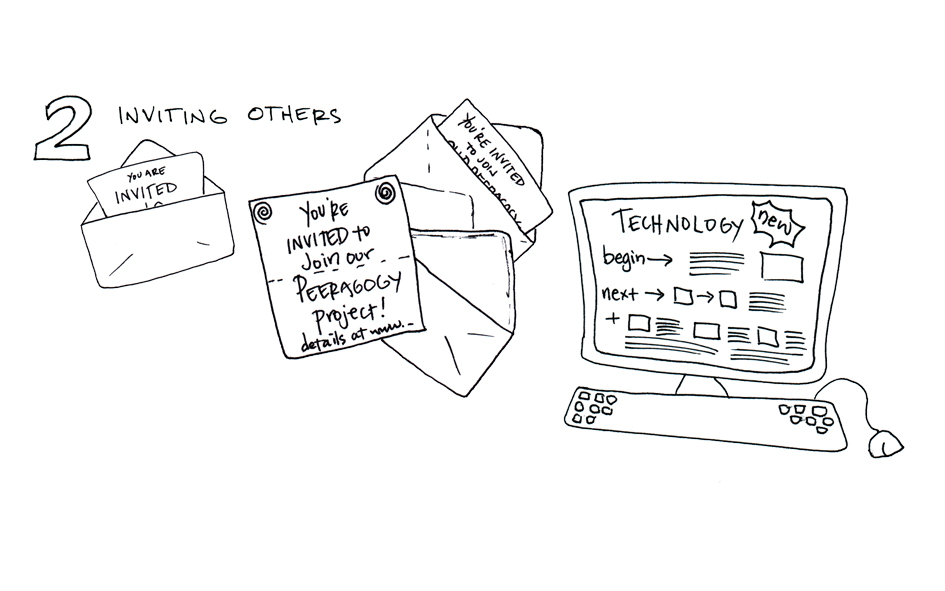
\includegraphics{./pictures/OpenBook-2-2.jpg}
\end{center}

\textbf{Other people can support you in achieving your goal and make the
work more fun too.}

\emph{Activity} -- Write an invitation to someone who can help with your
project. Clarify what you hope to learn from them and what your project
has to offer. Helpful questions to consider: What resources are
available or missing? What do you already have that you can build on?
How will you find the necessary resources? Who else is interested in
these kinds of challenges?

\emph{Technology} -- Pick a tool that's new to you and could potentially
be useful during the project. Start learning how to use it. Locate some
people around the world who share similar interests.

\emph{Suggested resources} -- The Peeragogy Handbook, parts III
(`\href{http://peeragogy.org/convening-a-group/}{Convening a Group}')
and IV
(`\href{http://peeragogy.org/organizing-a-learning-context/}{Organizing
a Learning Context}').

\emph{Recommended reading} -- Schmidt, J. Philipp. (2009). Commons-Based
Peer Production and education. Free Culture Research Workshop Harvard
University, 23 October 2009.

\emph{Observations from the Peeragogy project} -- We used a strategy of
`open enrolment': new people were welcome to join the project at any
time. We also encouraged people to either stay involved or leave --
several times over the past year, we required people to explicitly
reaffirm interest in order to stay registered in the forum and mailing
list. This choice cut down on `dead weight'. Nevertheless, the project
continued to accumulate content, which gave newcomers the discouraging
feeling that there was a lot to catch up on. We've aimed to sum up the
high points in the handbook!

\begin{center}
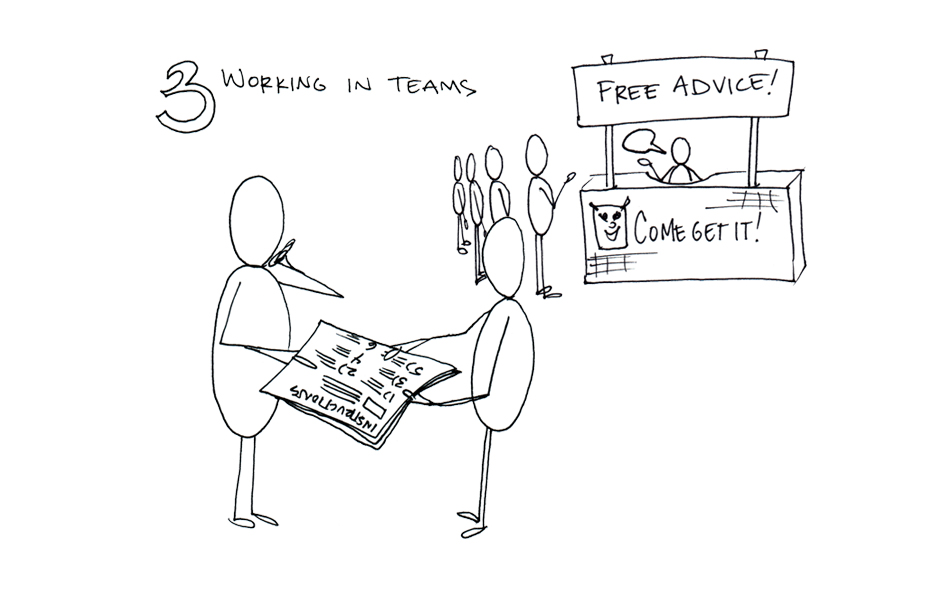
\includegraphics{./pictures/OpenBook-2-3.jpg}
\end{center}

\textbf{Solidifying your work plan and learning strategy together with
concrete measures for `success' can move the project forward
significantly. Working in teams and sharing information with others will
help you to develop your project.}

\emph{Activity} -- Concretise your ideas by, for example, writing an
essay, making visual sketches, or creating a short video to communicate
the unique plans for organisation and evaluation that your group will
use. Then, edit the pages of the Peeragogy Handbook boldly: by this time
you should have identified at least one section that needs to be
improved. Make the necessary revisions.

\emph{Technology} -- Take time to mentor others or be mentored by
someone, meeting up in person or online. Pair up with someone else and
share knowledge together about one or more tools. You can discuss some
of the difficulties that you've encountered, or teach a beginner some
tricks.

\emph{Suggested resources} -- The Peeragogy Handbook, parts V
(`\href{http://peeragogy.org/co-facilitation/}{Co-Facilitation and
Co-Working}'), VI
(`\href{http://peeragogy.org/assessment/}{Assessment}'), and part VII
(`\href{http://peeragogy.org/patterns-usecases/}{Patterns, Use cases,
and Examples}').

\emph{Recommended reading} -- Argyris, Chris. ``Teaching smart people
how to learn.'' Harvard Business Review 69.3 (1991); and, Gersick,
Connie J.G. ``Time and transition in work teams: Toward a new model of
group development.'' Academy of Management Journal 31.1 (1988): 9-41.

\emph{Observations from the Peeragogy project} -- Perhaps one of the
most important roles in the Peeragogy project was the role of the
`Wrapper', who prepared and circulated weekly summaries of forum
activity. This helped people stay informed about what was happening in
the project even if they didn't have time to read the forums. We've also
found that small groups of people who arrange their own meetings are
often the most productive.

\begin{center}
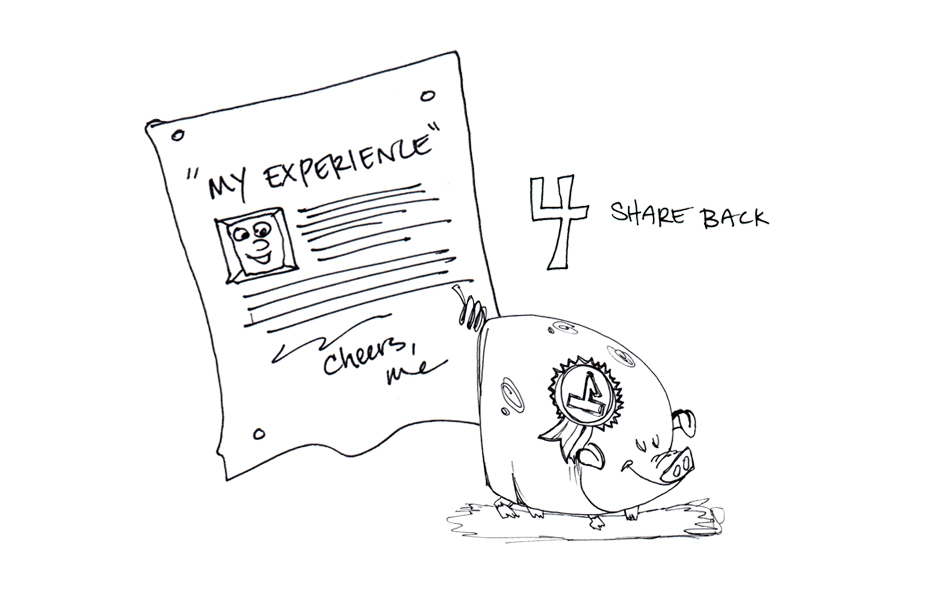
\includegraphics{./pictures/OpenBook-2-4.jpg}
\end{center}

\textbf{Wrap up the project with a critical assessment of progress and
directions for future work. Share any changes to this syllabus that you
think would be useful for future peeragogues!}

\emph{Activity} -- Identify the main obstacles you encountered. What are
some goals you were not able to accomplish yet? Did you foresee these
challenges at the outset? How did this project resemble or differ from
others you've worked on? How would you do things differently in future
projects? What would you like to tackle next?

\emph{Writing} -- Communicate your reflection case. Prepare a short
written (or video, or photo, \ldots{}) essay, dealing with your
experiences in this course. Share the results by posting it where others
in the broader Peeragogy project can find it.

\emph{`Extra credit'} -- Contribute back to one of the other
organisations or projects that helped you on this peeragogical journey.
Think about what you have to offer. Is it a bug fix, a constructive
critique, pictures, translation help, PR, wiki-gnoming or making a cake?
Make it something special, and people will remember you and thank you
for it.

\emph{Suggested resources} -- The Peeragogy Handbook, parts VIII
(`\href{http://peeragogy.org/resources/technologies/}{Technologies,
Services, and Platforms}') and IX
(`\href{http://peeragogy.org/resources/}{Resources}').

\emph{Recommended reading} -- Stallman, Richard.
"\href{http://www.gnu.org/philosophy/shouldbefree.html}{Why software
should be free}" (1992).

\emph{Observations from the Peeragogy project} -- When we were deciding
how to license our work, various Creative Commons licences were proposed
(CC Zero, CC By-SA and CC By-SA-NC). After a brief discussion, no one
was in favour of restricting downstream users, so we decided to use CC0.
In connection with this discussion, we agreed that we would work on ways
to explicitly build `reusability' into the handbook content.

\subsection{Micro-Case Study: The Peeragogy Project, Year 1}

Since its conception in early 2012, the Peeragogy Project has collected
over 3700 comments in our discussion forum, and over 200 pages of
expository text in the handbook. It has given contributors a new way of
thinking about things together. However, the project has not had the
levels of engagement that should be possible, given the technology
available and the global interest in improving education. We hope that
the handbook and this accompanying syllabus will provide a seed for a
new phase of learning, with many new contributors and new ideas drawn
from real-life applications.

\begin{center}
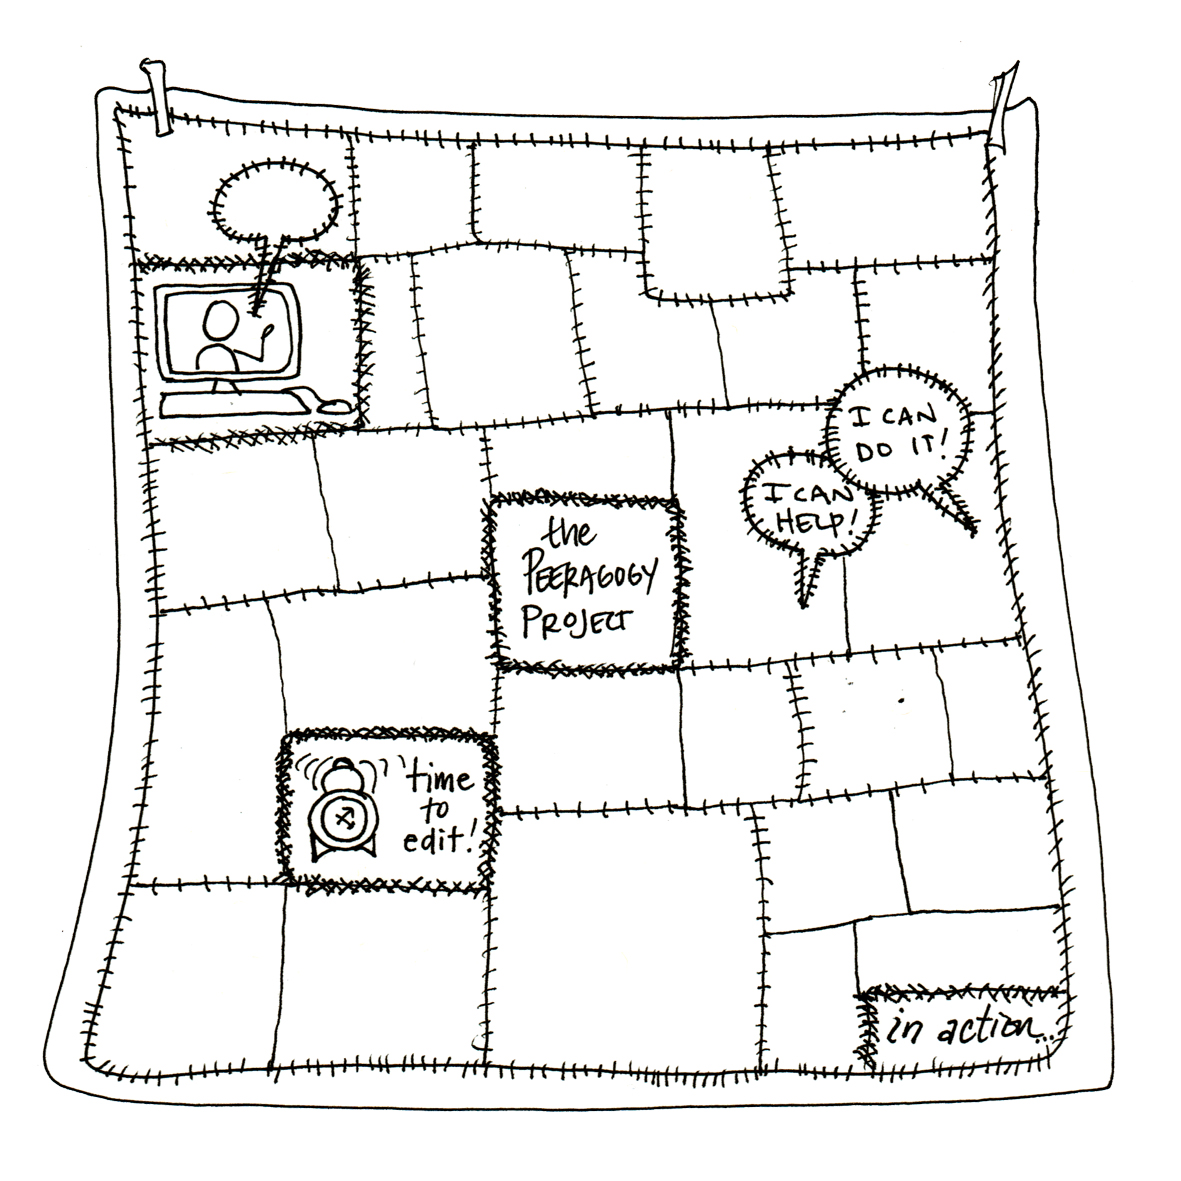
\includegraphics{./pictures/OpenBook-3.jpg}
\end{center}
